\begin{frame}
\frametitle{Breathing}
\begin{columns}[c] % The "c" option specifies centered vertical alignment while the "t" option is used for top vertical alignment

\column{.3\textwidth} % Left column and width
%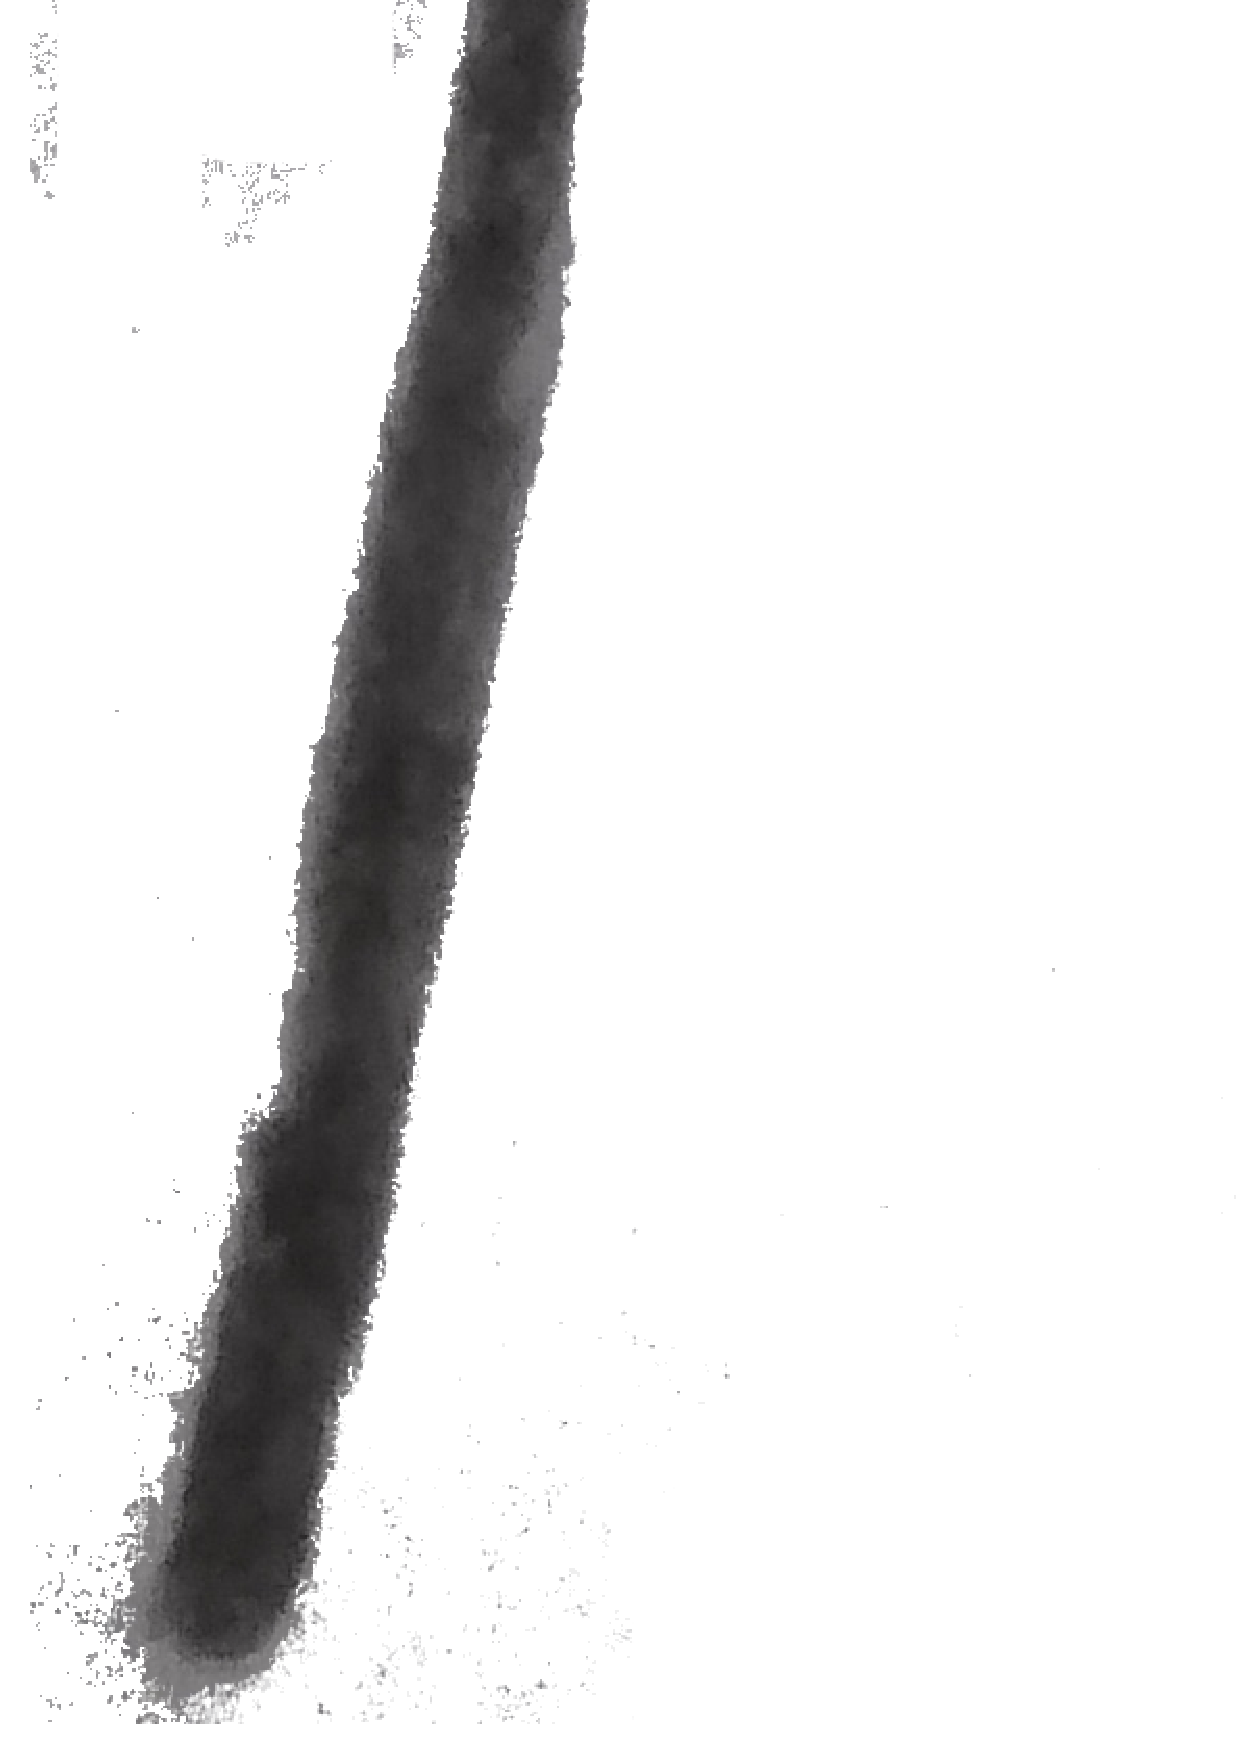
\includegraphics[width=\linewidth]{Sitting_chair_side.png}
\column{.7\textwidth} % Right column and width
\begin{itemize}
\item[-] I \structure{feel the crown}, the highest point of the head, I feel into it.
\item[-] I imagine how the \structure{breaths stream into my body through that point}, in a relaxed manner.
\item[-] And then I \structure{exhale through my feet}.
\item[-] Then I let the breath flow \structure{into my body through the feet} and \structure{out through the tip of my head}.
\end{itemize}
% Write on
\end{columns}
\end{frame}
%--------------------------------------------------------------------------------------------------------------

\begin{frame}
\frametitle{Observations}
\begin{columns}[c] % The "c" option specifies centered vertical alignment while the "t" option is used for top vertical alignment

\column{.3\textwidth} % Left column and width
%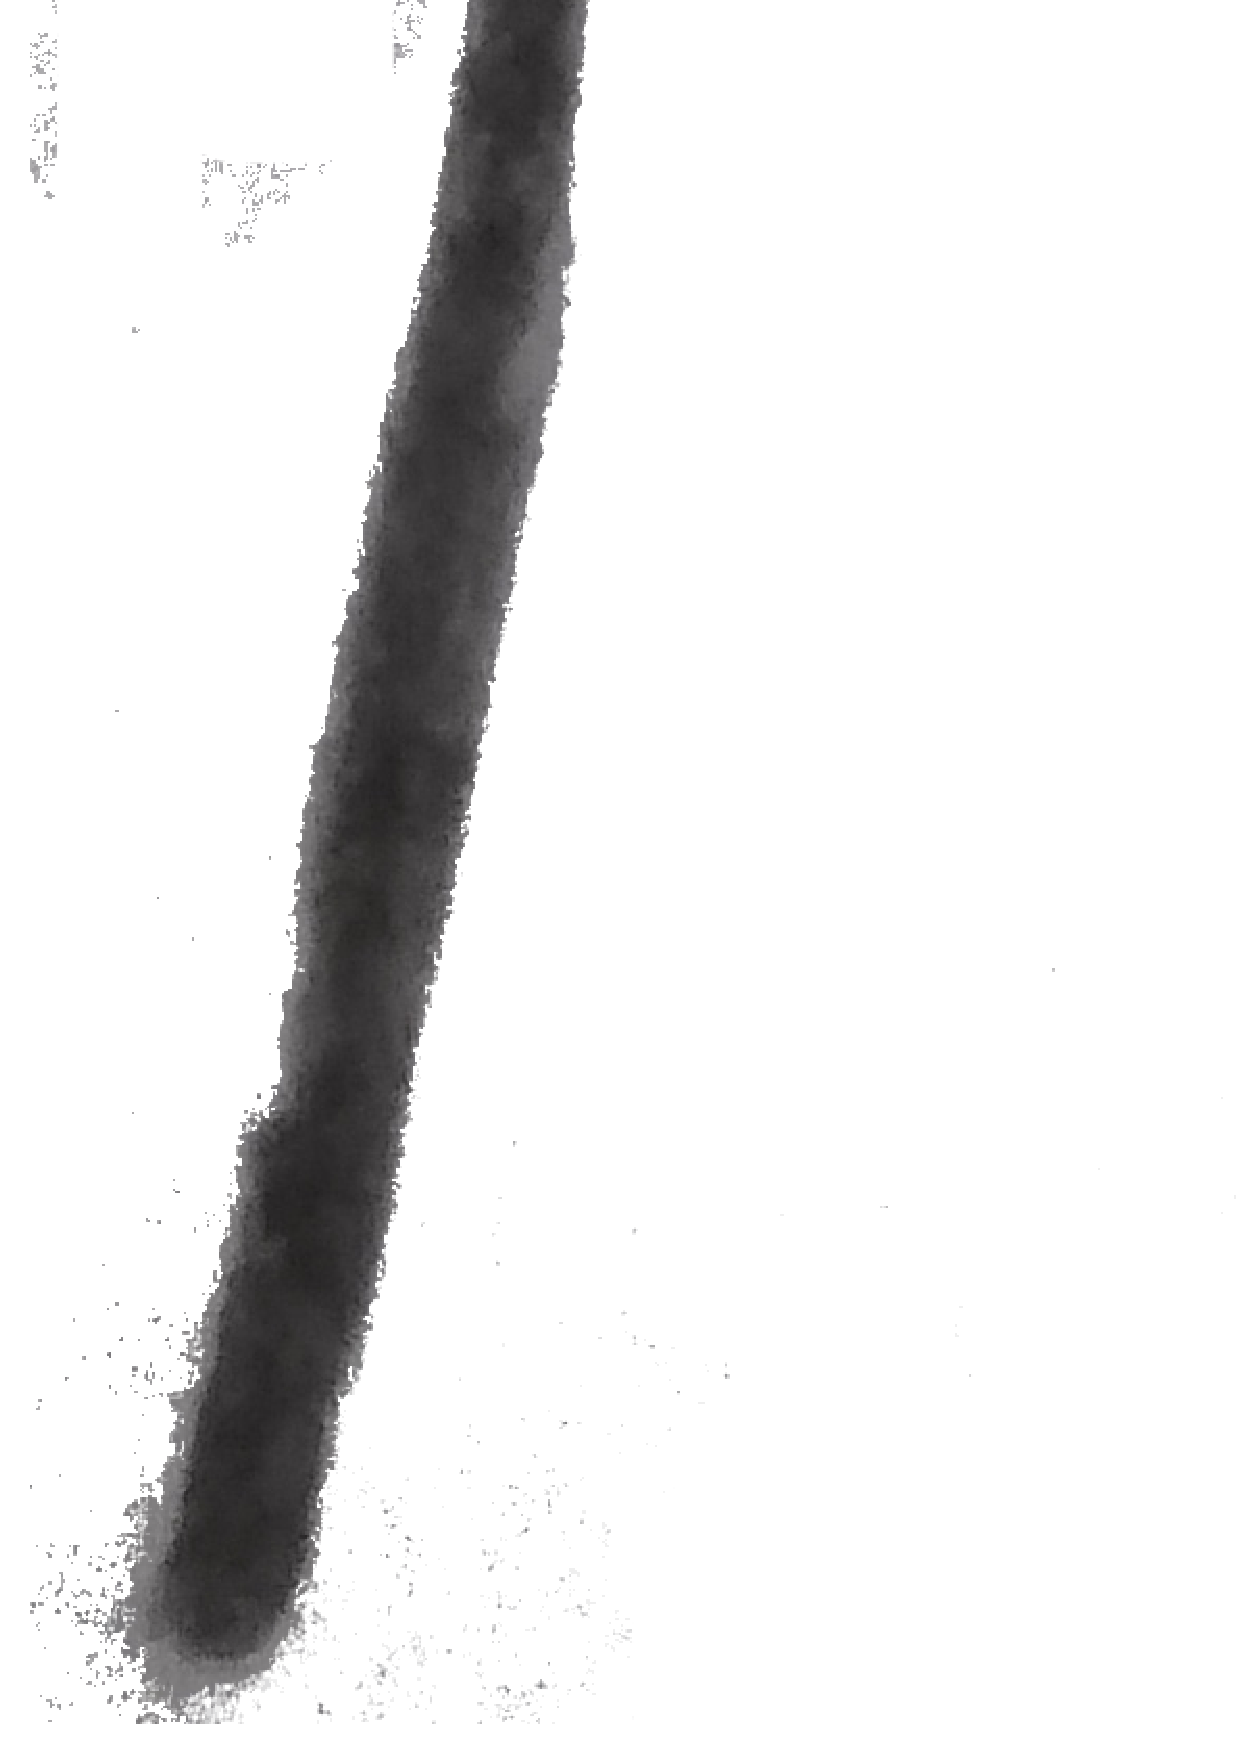
\includegraphics[width=\linewidth]{Sitting_chair_side.png}
\column{.7\textwidth} % Right column and width
\begin{itemize}
\item[-] I very attentively observe, \structure{how the breath flows} through my body.
\item[-] I'm totally present, I feel the \structure{body in it's entirety}, as a \structure{whole}.
\item[-] I feel myself as a whole.
\item[-] No worries, anxiety, discomfort can separate the whole thing that I am.
  \item[-] A feeling of \structure{deep joy and happiness} spreads throughout my whole body.

  \end{itemize}
% Write on
\end{columns}
\end{frame}
%--------------------------------------------------------------------------------------------------------------

\begin{frame}
\frametitle{Anchoring in the Here and Now}
\begin{columns}[c] % The "c" option specifies centered vertical alignment while the "t" option is used for top vertical alignment

\column{.3\textwidth} % Left column and width
%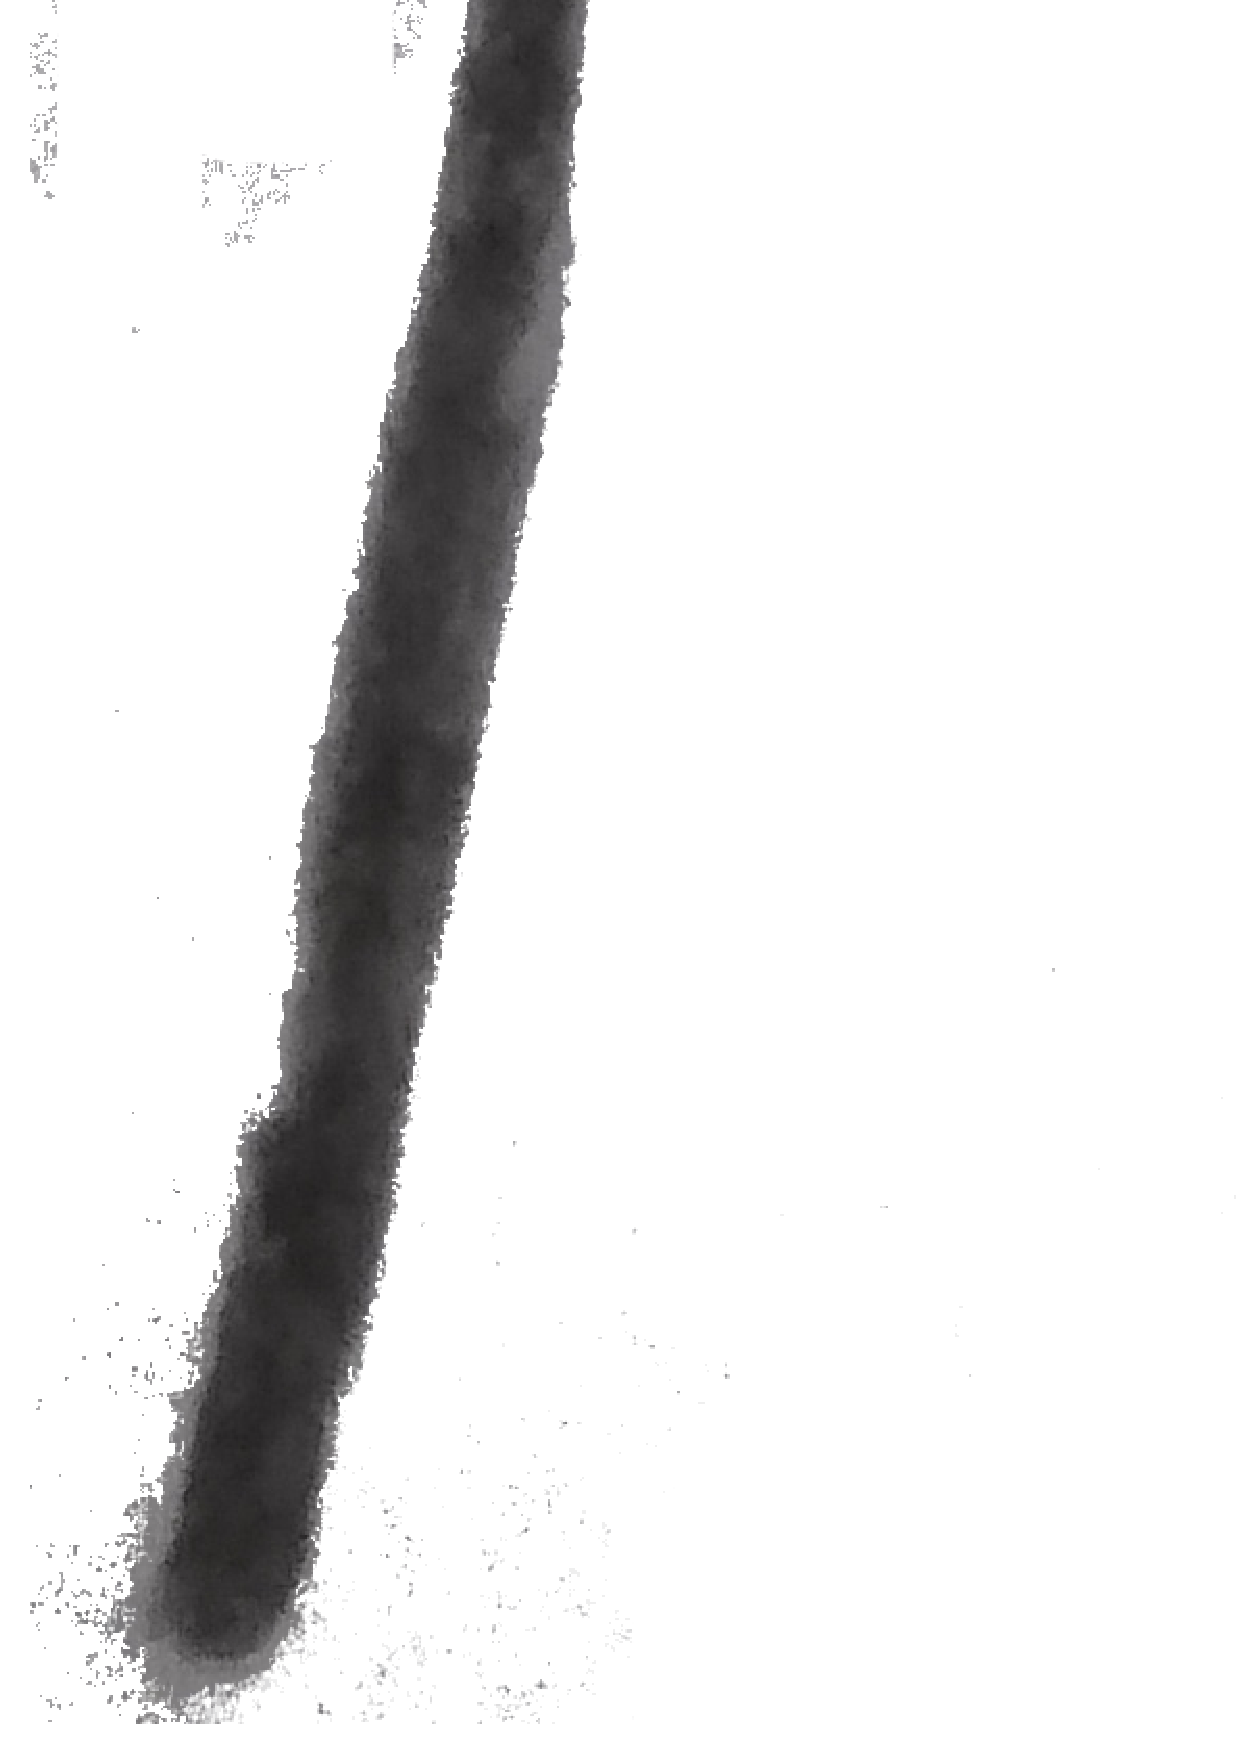
\includegraphics[width=\linewidth]{Sitting_chair_side.png}
\column{.7\textwidth} % Right column and width
\begin{itemize}
\item[-] Now, I direct my attention again to \structure{my body}, the space and am back in the \structure{here and now}.
  \item[-] I keep the \structure{peace} and the \structure{deep happiness} inside of me and am happy to be the way I am.
\end{itemize}
% Write on
\end{columns}
\end{frame}
%--------------------------------------------------------------------------------------------------------------

\begin{frame}
\frametitle{Returning}
\begin{columns}[c] % The "c" option specifies centered vertical alignment while the "t" option is used for top vertical alignment

\column{.3\textwidth} % Left column and width
%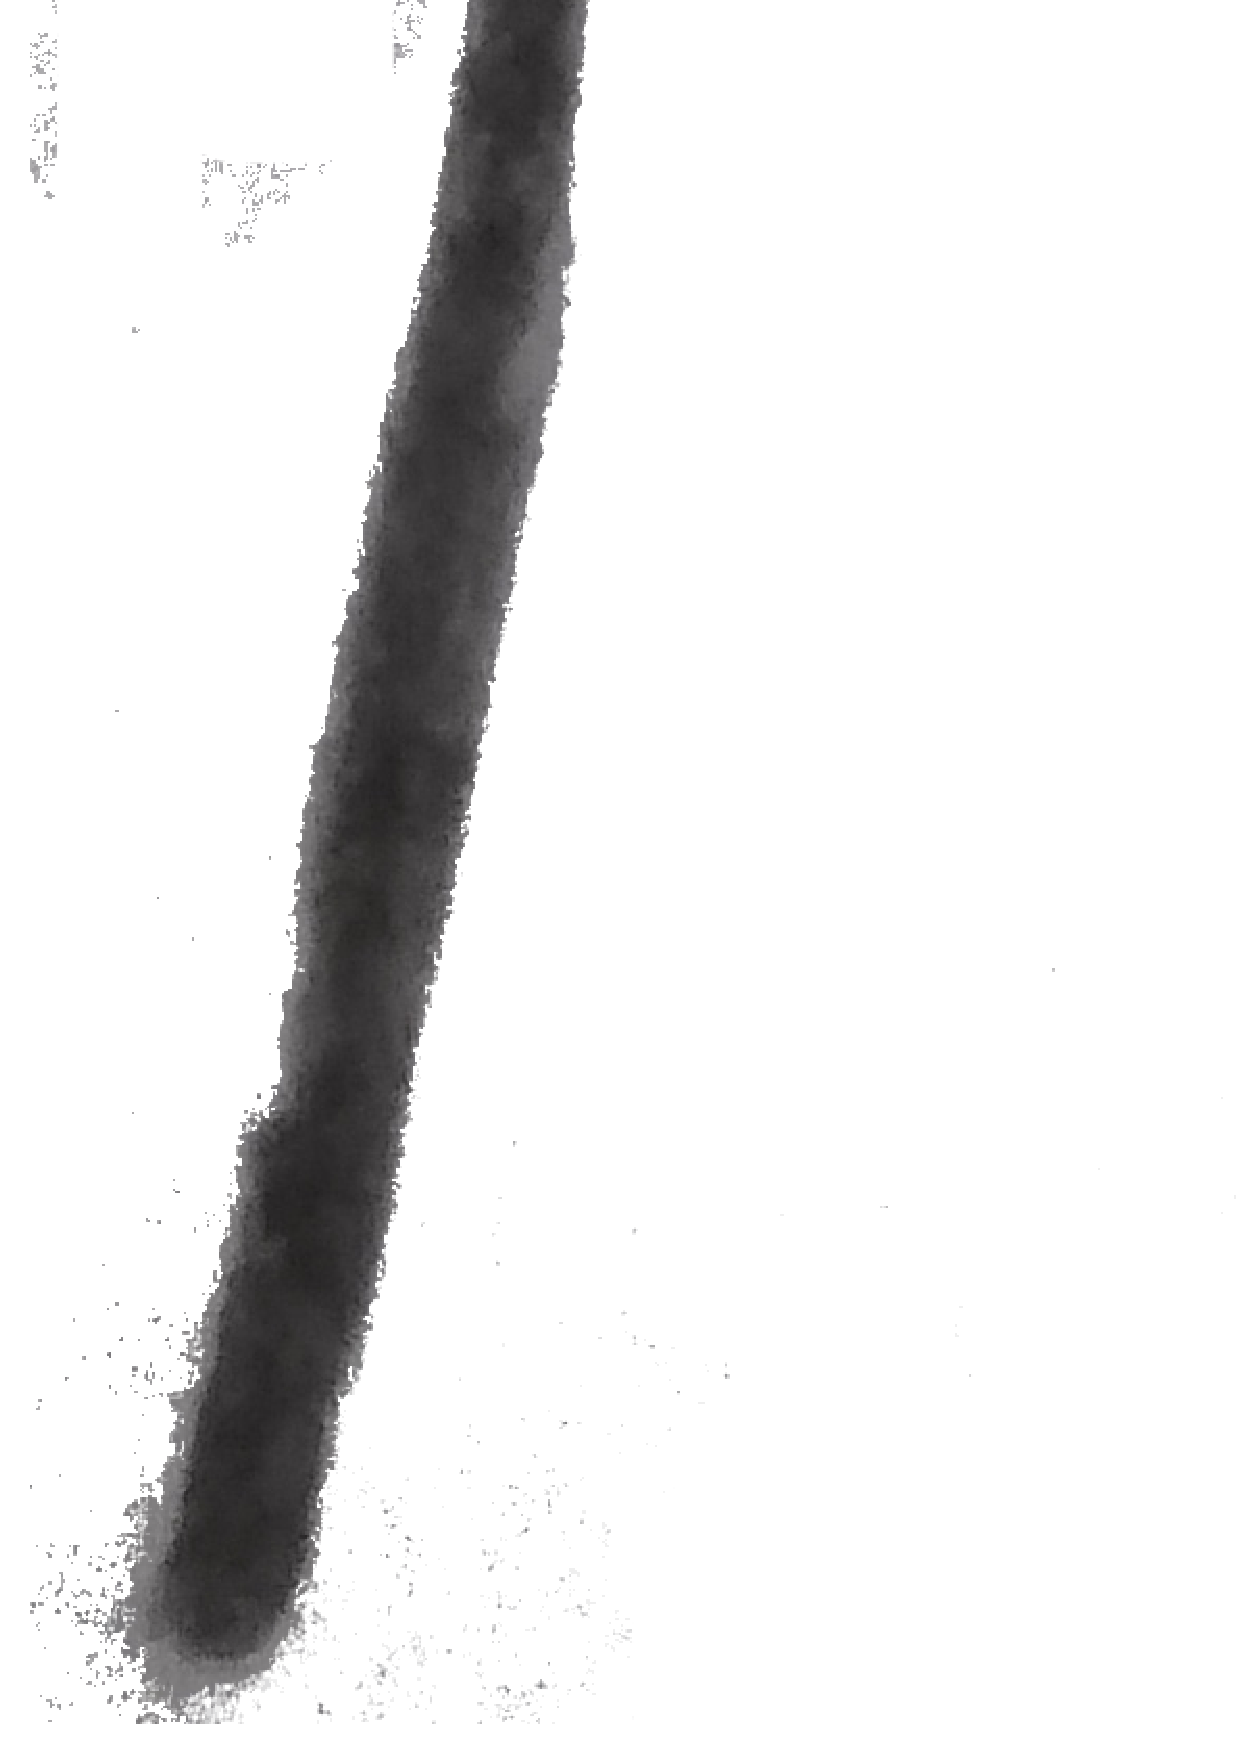
\includegraphics[width=\linewidth]{Sitting_chair_side.png}
\column{.7\textwidth} % Right column and width
\begin{itemize}
\item[-] I \structure{count from 7 to 1} and am \structure{totally back here}.
\item[-] I lightly \structure{move} my finger, the hands, slowly open my eyes and slowly roll the head back and forth.
  \item[-] I stretch with pleasure my limbs.
  \end{itemize}
% Write on
\end{columns}
\end{frame}
%--------------------------------------------------------------------------------------------------------------
